\section{Foundational Concepts for Mechanistic Interpretability}
\label{sec:foundations}

This section introduces foundational concepts in mechanistic interpretability. We establish a shared notation and vocabulary for use throughout the survey. We avoid committing to specific hypotheses about the representations and workings of model activations. 

\subsection{Behavioural vs.\ Mechanistic Understanding}
\label{subsec:behavioral-vs-mechanistic}

Behavioural analysis describes what a model does, but safety-critical applications also require understanding its internal mechanism (as we reviewed in Section~\ref{sec:why_open}).

\begin{definitionbox}[Behavioural Interpretability]
Behavioural interpretability studies a model $f_\theta : \mathcal{X} \to \mathcal{Y}$
through input--output pairs $(x, f_\theta(x))$ for $x \in \mathcal{D} \subseteq \mathcal{X}$,
where $\mathcal{D}$ is a finite test set. Behavioural interpretability treats the model as a black box.
\end{definitionbox}


\begin{definitionbox}[Mechanistic Interpretability]
Mechanistic interpretability studies a model $f_\theta : \mathcal{X} \to \mathcal{Y}$ by examining
its internal computations, including model activations and parameters $\theta$ that produce them, at different levels of granularity in relation to its behaviour. In short, mechanistic interpretability characterises how a model's behaviour or output is computed.

\end{definitionbox}

\subsection{Neuron Polysemanticity in Model Representations}
\label{subsec:polysemanticity}

\paragraph{What Is a Concept?}
Concepts play a central role in many interpretability methods and will be used throughout this paper to define key ideas such as features and polysemanticity. It is therefore worth clarifying what we mean by the term. Notably, concepts do not necessarily correspond to categories humans can readily name or understand; neural networks may represent them in ways humans lack the vocabulary to describe~\citeest{hewitt2025position}.

\begin{definitionbox}[Concept]
A concept is a distinct, reusable unit of information or knowledge that can be identified across different instances or contexts. Concepts may correspond to familiar human categories, such as ``a dog'', ``the colour red'', or ``words of praise'', but they need not admit a natural human description.
\end{definitionbox}

Cross-context identifiability concerns the meaning of the information unit rather than the process by which the information is recognised. Determining whether a concept is present in an information unit may itself require additional contextual information. For example, the word (i.e., an instance of an information unit) ``bank'' can refer to a financial institution or a river bank, depending on the surrounding sentence. Nevertheless, once identified, each concept can be recognised as the same information across different contexts. For example, the concept of ``financial institution'' is expected to remain sufficiently stable across the contexts in which it appears.

This definition accommodates both human-interpretable and machine-specific concepts. A machine-specific concept may lack a natural human description yet still form a coherent, reusable unit of information in the neural network~\citeest{dalvi2022discovering, hewitt2025position}. Human interpretability should therefore be treated as a property of some concepts rather than as a necessary condition for the information unit to qualify as a concept. Notably, most interpretability research focuses on concepts that humans can readily understand. Identifying and characterising concepts that matter to a model's computation but do not map neatly onto human-understandable categories remains underexplored.

\paragraph{Neuron Polysemanticity.}
For a single neuron $n_\ell$ in layer $\ell$, consider its activation at token position $t$ for some input prompt $x$, denoted by $n_\ell^{t}(x)$. We can straightforwardly interpret a neuron if it responds to a single concept. For example, if $n_\ell^{t}(x)$ is large and positive whenever position $t$ corresponds to the word ``blue'', remains close to zero otherwise, and can causally shift the model's outputs towards or away from blue-related concepts when manipulated, we can conclude that the neuron corresponds to the concept of blue. Assuming some neurons exhibit such a property, early work proposed methods to discover and interpret individual neurons' functions~\citeest{netdissect2017, bau2018identifying, Dalvi_Durrani_Sajjad_Belinkov_Bau_Glass_2019, bau2020units, hernandez2022natural, oikarinen2023clipdissect, and}. However, follow-up studies have found that, due to representational constraints and superposition~\citeem{elhage2022superposition} (detailed in Section~\ref{subsec:superposition}), individual neurons often respond strongly to multiple concepts that appear unrelated from a human perspective~\citeem{elhage2022superposition}. This phenomenon is known as \textit{neuron polysemanticity}.



\begin{definitionbox}[Neuron Polysemanticity]
A neuron $n_\ell$ is \emph{polysemantic} if there exist two distinct concepts $c_1$ and $c_2$, together with corresponding sets of inputs $x_1$ and $x_2$ as well as token positions of interest $t_{c_1}$ and $t_{c_2}$, such that $n_\ell^{t_{c_1}}(x_1)$ and $n_\ell^{t_{c_2}}(x_2)$ are both large, and interventions on these activations causally influence model behaviour associated with both concepts.

\end{definitionbox}

Polysemanticity complicates neuron-level explanations and suggests that human-interpretable semantic content may not be aligned with individual neurons. This motivates searching for representational units beyond individual neurons.

\subsection{Features as Representational Units}
\label{subsec:features}

Since individual neurons are often polysemantic, mechanistic interpretability has increasingly shifted towards alternative units of analysis. For example, it has been found that models sometimes encode human-interpretable concepts as linear directions or low-dimensional manifolds in the activation space~(\citeestalp{arditi2024refusallanguagemodelsmediated}; \citeemalp{wurgaft2026manifoldsteeringrevealsshared}). We thus use the term \emph{feature} broadly to encompass any model representation corresponding to a human-interpretable concept. Such distributed representations motivate analysing the activation space as a whole, rather than individual neurons in isolation~\citeem{elhage2022superposition, bricken2023monosemanticity, templeton2024scaling}.

Specifically, we treat a feature technically as a geometric structure $\phi$ in the activation space $\mathbb{R}^d$ of a model component, such as the residual stream, an attention-head output, or an MLP output, where $d$ denotes the hidden dimension. Conceptually, a feature is a manipulable manifestation of a concept of interest. As with neurons, for a feature $\phi$ claimed to correspond to a concept $c$, we expect interventions that increase or suppress the activation of $\phi$ to causally influence model behaviour associated with $c$. In this sense, features provide a more expressive, general representational unit than individual neurons for describing how neural networks may encode concepts.

\begin{definitionbox}[Feature]
A feature $\phi$ associated with a concept $c$ is a geometric structure in the model's activation space $\mathbb{R}^d$ whose activation is predictive of, and causally relevant to, the presence or expression of $c$.
\end{definitionbox}


At this stage, we remain agnostic about the precise mathematical form features take and how the model encodes them. Instead, we treat existing methods for identifying and manipulating features as operational approximations shaped by their methodological assumptions and constraints. We examine these representational hypotheses explicitly in Section~\ref{sec:hypotheses}.

Within this operational perspective, researchers can identify features using several methodological families, including readout-based methods~\citeest{patchscopes, pan2024latentqateachingllmsdecode, ao} and sparse decomposition techniques~\citeest{cunningham2023sparse, dunefsky2024transcodersinterpretablellmfeature}, and then manipulate them to test causal relevance~\citeest{wu2025axbench, mueller2025mib}. In practice, many such approaches operationalise features as approximately linear or linearised components of internal representations~(\citeemalp{yun-etal-2021-transformer}; \citeestalp{marks2024the, arditi2024refusallanguagemodelsmediated}). Examples include linear probes and dictionary-learning methods~(\citeestalp{belinkov-2022-probing}; \citeemalp{bricken2023monosemanticity}).

An important caveat is that, for a given concept, an identified manipulable geometric structure---that is, a candidate feature---may be only one of many possible internal representations associated with that concept. For example, a language model may encode the concept of ``refusal'' in a complex manner across multiple layers and components. Successfully identifying a linear direction in the residual stream that can steer the model towards or away from refusal~\citeest{arditi2024refusallanguagemodelsmediated} does not imply that this direction uniquely or exhaustively captures how refusal is represented. Other causally relevant structures (e.g., low-dimensional manifolds) for refusal may also exist but remain unidentified.

\subsection{Transformer Computation}
\label{subsec:transformers}

Transformers~\citeest{vaswani2017attention} have become the dominant architecture underlying modern language-model-based AI assistants such as ChatGPT and Claude, and are consequently the primary subject of study in mechanistic interpretability. Several properties of the transformer architecture, most notably its modular structure and additive information flow, make it particularly amenable to mechanistic analysis~\citeem{elhage2021mathematical}. In particular, transformer components can be viewed as reading from and writing to a shared \emph{residual stream}, allowing information to persist and be incrementally transformed as it passes through successive layers~\citeem{elhage2021mathematical}. Below, we briefly review the main classical components of the transformer architecture.




\begin{definitionbox}[Residual Stream and Computational Components]
Let
\[
h^{1:T}_\ell(x) \in \mathbb{R}^{d \times T}
\]
denote the sequence of residual-stream activations at layer $\ell$ for an input
sequence $x$, where $T$ is the sequence length and $d$ is the model hidden size.
The residual stream serves as the shared communication channel through which
transformer components exchange information. Below, in this box, we let $h_\ell(x) \coloneqq h^{1:T}_\ell(x)$ to simplify the notation.\\

For a standard transformer layer $\ell$, consisting of a multi-head attention module $\mathrm{Attn}_\ell(\cdot)$ and a multi-layer perceptron $\mathrm{MLP}_\ell(\cdot)$, we have
\begin{align*}
h'_\ell(x)
    &= h_{\ell-1}(x)
       + \mathrm{Attn}_\ell(h_{\ell-1}(x)), \\
h_\ell(x)
    &= h'_\ell(x)
       + \mathrm{MLP}_\ell(h'_\ell(x))
    = h_{\ell-1}(x)
       + \mathrm{Attn}_\ell(h_{\ell-1}(x)) + \mathrm{MLP}_\ell(h'_\ell(x)).
\end{align*}

Unrolling the recursion gives
\[
h_\ell(x)
=
h_0(x)
+
\sum_{k=1}^{\ell}
\Big(
\mathrm{Attn}_k(h_{k-1}(x))
+
\mathrm{MLP}_k(h'_k(x))
\Big),
\]

where \(h_0(x)\) denotes the input embedding representation. The equation shows that the residual stream at layer \(\ell\) equals the input embeddings plus the accumulated outputs of all computational components that have written to the residual stream up to that point. This perspective is central to mechanistic interpretability, as it lets us decompose model computation into additive contributions from individual components~\citeem{elhage2021mathematical}.

\end{definitionbox}







For simplicity, we omit layer-normalisation operations from the notation. Following \citetem{elhage2021mathematical}, most of the layer-normalisation transformation can be absorbed into adjacent linear components. Specifically, for a fixed input, layer normalisation is well approximated as an affine transformation with a scalar rescaling factor. The affine part can be folded into neighbouring parameters, and the remaining scalar normalisation term simply reweights component contributions. This approximation lets us treat the residual stream as an additive communication channel without explicitly representing normalisation at every layer.

Attention heads and MLPs play distinct roles in transformer computation. Attention modules primarily route, aggregate, and compose information across token positions~(\citeemalp{olsson2022incontextlearninginductionheads}; \citeestalp{wang2022interpretabilitywildcircuitindirect}), whereas MLPs often perform feature transformation and factual knowledge retrieval~\citeest{geva-etal-2021-transformer, meng2023locatingeditingfactualassociations}. This functional separation enables more localised analyses of how the model routes, transforms, and stores information, as well as how attention modules and MLPs interact~\citeest{neo-etal-2024-interpreting}.

Below, we detail the computations of canonical attention modules and MLPs.

\begin{definitionbox}[Attention Module]

A multi-head attention module consists of $N_H$ attention heads operating in parallel. Consider the residual-stream activations $ h_\ell^{1:T}(x) \in \mathbb{R}^{d \times T}$ and let $h := h_\ell^{1:T}(x)$ for notational simplicity. For each head $r \in \{1,\ldots,N_H\}$, the residual stream is first projected into query, key, and value representations:
\[
Q^r = W_Q^r h,
\qquad
K^r = W_K^r h,
\qquad
V^r = W_V^r h,
\]
where $W_Q^r, W_K^r, W_V^r \in \mathbb{R}^{d_{\text{head}} \times d}$ and $d_{\text{head}}$ denotes the dimensionality of each attention head. The \emph{attention pattern} of head $r$ is then computed as
\[
A^r
=
\operatorname{softmax}\!\left(
\frac{(Q^r)^\top K^r}{\sqrt{d_{\text{head}}}}
\right)
\in
\mathbb{R}^{T \times T},
\]
where the softmax is applied row-wise. Thus, $A^r_{t,t'}$ denotes the attention weight assigned by the query at position $t$ to the key at position $t'$. The head then writes an update to the residual stream:
\[
\Delta h^r
=
W_O^r V^r (A^r)^\top,
\]
where $W_O^r \in \mathbb{R}^{d \times d_{\text{head}}}$. The output of the full multi-head attention module is the sum of the contributions from all heads:
\[
\operatorname{Attn}(h)
=
\sum_{r=1}^{N_H}
\Delta h^r.
\]

\end{definitionbox}


\begin{definitionbox}
[MLP Block]
An MLP block applies a position-wise nonlinear transformation to each position of the residual stream. In the canonical transformer architecture~\citeest{vaswani2017attention}, this transformation takes the form
\[
\Delta h_{\text{MLP}} = W_2 \,\sigma(W_1h+b_1)+b_2,
\]
where $W_1 \in \mathbb{R}^{d_{\text{mlp}}\times d}$, $W_2 \in \mathbb{R}^{d\times d_{\text{mlp}}}$, and $\sigma(\cdot)$ denotes a nonlinear activation function, for which the original transformer uses ReLU~\citeest{relu}. The same transformation is applied independently at each position in the sequence. MLP blocks primarily
transform and generate internal features, writing new directions into the
residual stream.\\

Notably, $W_1$ typically projects the activations into a much higher-dimensional space ($d_{\text{mlp}} \gg d$), which has recently been found to yield more interpretable representations natively in the model~\citeest{ICLR2025_8c5f3029, arora2026language}.

\end{definitionbox}

The transformer components discussed above correspond to their canonical formulations. Numerous variants have since been proposed and adopted in modern architectures. For example, variants of the attention module include Grouped Query Attention (GQA)~\citeest{gqa}, used in Llama 3~\citeem{llama3}, and Multi-Head Latent Attention (MLA)~\citeem{deepseekv2}, used in DeepSeek-V2~\citeem{deepseekv2} and DeepSeek-V3~\citeem{deepseekai2025deepseekv3technicalreport}. Variants of the MLP block include gated architectures such as SwiGLU~\citeem{shazeer2020gluvariantsimprovetransformer}, used in Llama 3, and Mixture-of-Experts (MoE) architectures, used in DeepSeek-V3.



\subsection{Circuits as Descriptions of Internal Mechanisms}
\label{subsec:circuits}

Sections~\ref{subsec:polysemanticity}--\ref{subsec:features} introduce neurons and features as representational units for describing what is represented in model activations, and Section~\ref{subsec:transformers} introduces the computations that transform and route activations through the model. We use the term \emph{mechanism} to refer to the organisation of model activations, their representational units, or the transformations applied to them that together produce a particular model behaviour. A central topic in mechanistic interpretability is identifying and understanding such mechanisms in neural networks.

A common way to represent and describe such a mechanism is through a \emph{circuit}: a subgraph of the model's computational graph whose \emph{nodes} correspond to computational components or representational units and whose \emph{edges} represent information flow between them~\citeem{elhage2021mathematical}.

\begin{definitionbox}[Circuit (Figure~\ref{fig:circuit})]
For a fixed model computation, let \(G\) denote the corresponding directed acyclic computational graph. A circuit \(\mathcal{C} \subseteq G\) is a subgraph of \(G\), where:
\begin{itemize}[nosep]
    \item \textbf{Nodes:} computational components, such as \(\mathrm{Attn}_\ell\) and \(\mathrm{MLP}_\ell\), or representational units, such as features \(\phi_i\);
    \item \textbf{Edges:} directed connections representing information flow or transformation between nodes.
\end{itemize}
The subgraph \(\mathcal{C}\) represents a collection of components and interactions that jointly contribute to a particular computation or model behaviour, and can therefore serve as a description of the underlying mechanism.
\end{definitionbox}

\begin{figure}[tb]
  \centering
  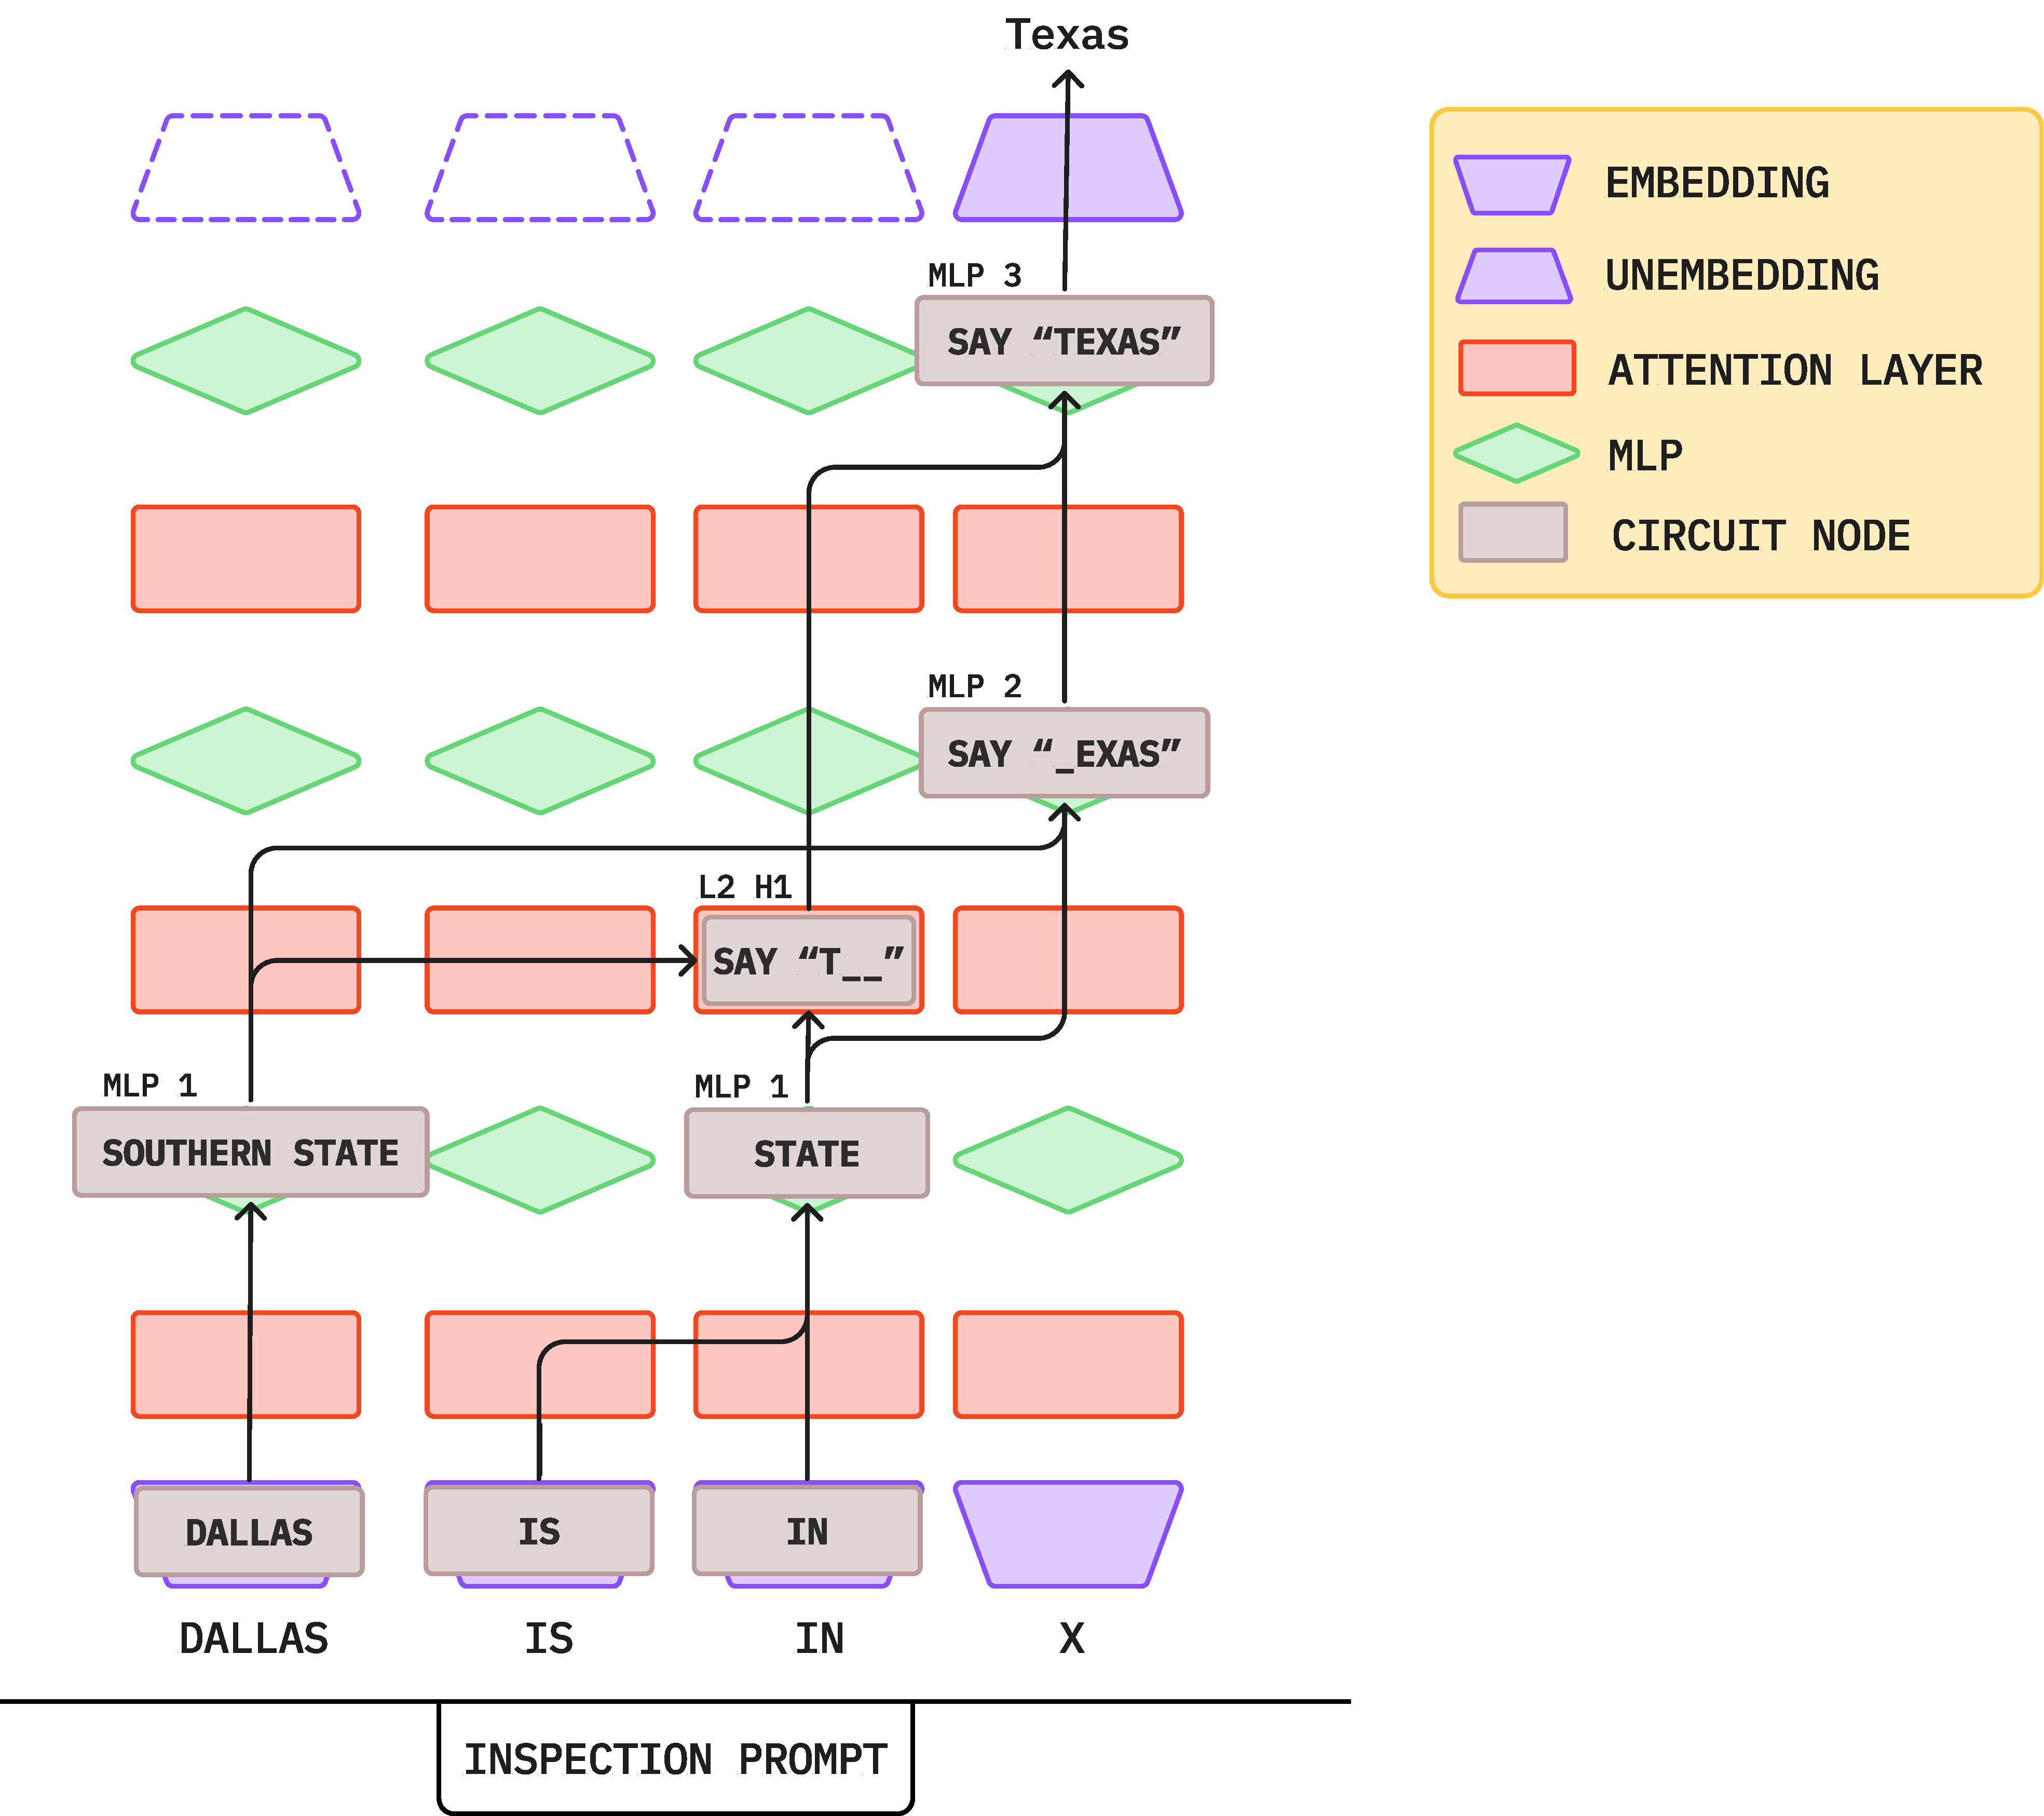
\includegraphics[width=0.7\textwidth]{figs/7_Circuit.pdf}
  \caption{\textbf{Circuit.} This diagram illustrates a circuit within a transformer, where specific nodes (MLP layers and attention heads in this case) perform specialised computations.}
  \label{fig:circuit}
\end{figure}

\begin{examplebox}[Examples of Circuits]
\begin{itemize}
    \item \textbf{Induction head circuit:} Two attention heads cooperate to implement in-context learning~\citeem{olsson2022incontextlearninginductionheads}.
    \item \textbf{QK circuits:} Query--Key interactions prioritising specific token positions~\citeem{kamath2025tracing}.
\end{itemize}
\end{examplebox}

The study of circuits has developed along two complementary lines. The first line of work~\citeest{wang2022interpretabilitywildcircuitindirect, conmy2023automatedcircuitdiscoverymechanistic, eapig, haklay-etal-2025-position}, referred to as \emph{capability circuit discovery} by \citetest{querycircuit}, aims to identify minimal sets of architectural components, such as attention heads or MLP layers, that are sufficient to reproduce a given \textit{behaviour} or \textit{capability} of the model, such as indirect object identification~\citeest{wang2022interpretabilitywildcircuitindirect}, numerical comparison~\citeest{hanna2023how}, and in-context learning~\citeest{kharlapenko2025scaling}. In this setting, the capability of interest is defined as a dataset of queries that exercise it, and a discovered circuit is considered successful if it recovers the model's performance on this dataset.


The second line of work, referred to as \emph{query-level circuit discovery}~\citeest{querycircuit}, focuses on how internal features interact and propagate across the computational graph to produce the model's decision for a particular input query~(\citeemalp{ameisen2025circuit}; \citeestalp{querycircuit}). Studies in this line usually use sparse autoencoders or cross-layer transcoders (detailed in Section~\ref{sec:sae}) to automatically decompose MLP outputs into interpretable units, trace attributions between these features, and track how information flow converges to the final prediction. 

\paragraph{Summary.}
This section introduced the foundational concepts of mechanistic interpretability: neuron polysemanticity, which motivates the use of features as more expressive units of analysis; transformer computation, which describes how representations are transformed and information is routed through the model; and internal mechanisms, which organise these units, transformations, and information flows to produce model behaviour and can be described by circuits. How we interpret and leverage these concepts depends on assumptions about the structure of model representations and computation, which we examine explicitly in Section~\ref{sec:hypotheses}.



